\begin{frame}[fragile]
    \frametitle{version control}
\begin{center}
    \normalsize
    Ephemeral vs Persistent Data Structures


    
    \note{To provide version control capabilities on data, we first delve into the theory of persistent data structures.
    A data structure that does NOT provide access to its history is called an ephemeral data structure.
    All changes to an ephemeral data structure occur in-place and only the most recent version is ever available.
    An example of an ephemeral data structure are those found in the Java Collections Framework.
    (Add an image here??)
    
    On the other hand, a persistent data structure provides access to different versions of a similar---in the sense of expected operations---ephemeral data structure.
    The data structure starts at an initial version, and any subsequent updates creates new versions of the data structure.}


    \pause

    Types of persistence:

    \begin{tabular}{l  l}
        \pause
        \textbf{Partial Persistence} &
        \adjustbox{margin=0.1cm}{
          \resizebox{0.35\linewidth}{!}{
              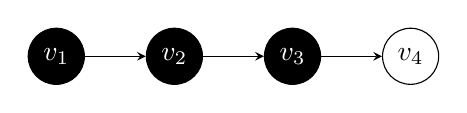
\begin{tikzpicture}[baseline={([yshift=-14pt]current bounding box.north)}]
              \begin{scope}[>=stealth]
                \node (v1) at (0,0) [circle,draw,style={fill=black, text=white}]{$v_1$};
                \node (v2) at (1.5,0) [circle,draw,style={fill=black, text=white}]{$v_2$};
                \node (v3) at (3,0) [circle,draw,style={fill=black, text=white}]{$v_3$};
                \node (v4) at (4.5,0) [circle,draw]{$v_4$};

                \draw[->] (v1) -- (v2);
                \draw[->] (v2) -- (v3);
                \draw[->] (v3) -- (v4);

              \end{scope}
              \end{tikzpicture}
          }
        }

        \\
        % \hline

        \pause
        \normalsize \textbf{Full Persistence} &
        \adjustbox{margin=0.1cm}{
          \resizebox{0.35\linewidth}{!}{
          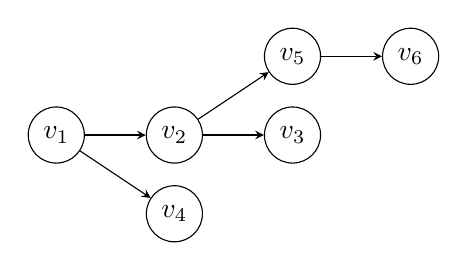
\begin{tikzpicture}[baseline={([yshift=-42pt]current bounding box.north)}]
          \begin{scope}[>=stealth]
            \node (v1) at (0,0) [circle,draw]{$v_1$};
            \node (v2) at (1.5,0) [circle,draw]{$v_2$};
            \node (v3) at (3,0) [circle,draw]{$v_3$};
            \node (v4) at (1.5,-1) [circle,draw]{$v_4$};
            \node (v5) at (3,1) [circle,draw]{$v_5$};
            \node (v6) at (4.5,1) [circle,draw]{$v_6$};

            \draw[->] (v1) -- (v2);
            \draw[->] (v1) -- (v4);
            \draw[->] (v2) -- (v3);
            \draw[->] (v2) -- (v5);
            \draw[->] (v5) -- (v6);

          \end{scope}
          \end{tikzpicture}
          }
        } \\

        % \hline
        \pause
        \normalsize \textbf{Confluent Persistence} &
        \adjustbox{margin=0.1cm}{
        \resizebox{0.35\linewidth}{!}{
        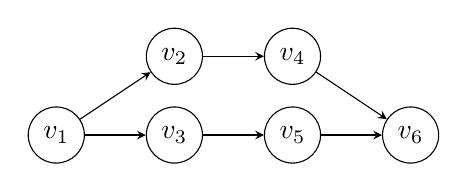
\begin{tikzpicture}[baseline={([yshift=-26pt]current bounding box.north)}]
        \begin{scope}[>=stealth]

          \node (v1) at (0,0) [circle,draw]{$v_1$};
          \node (v2) at (1.5,1) [circle,draw]{$v_2$};
          \node (v3) at (1.5,0) [circle,draw]{$v_3$};
          \node (v4) at (3,1) [circle,draw]{$v_4$};
          \node (v5) at (3,0) [circle,draw]{$v_5$};
          \node (v6) at (4.5,0) [circle,draw]{$v_6$};

          \draw[->] (v1) -- (v2);
          \draw[->] (v1) -- (v3);
          \draw[->] (v2) -- (v4);
          \draw[->] (v3) -- (v5);
          \draw[->] (v5) -- (v6);
          \draw[->] (v4) -- (v6);

        \end{scope}
        \end{tikzpicture}
        }}
    \end{tabular}
\end{center}

\end{frame}